\documentclass[9pt,twocolumn,twoside]{gsajnl_modified}
% Use the documentclass option 'lineno' to view line numbers

\usepackage[htt]{hyphenat}  % https://tex.stackexchange.com/a/543
\usepackage[export]{adjustbox}
\usepackage{xurl}
\usepackage{stfloats}
\usepackage[leftcaption]{sidecap}
\sidecaptionvpos{figure}{t}

\renewcommand{\topfraction}{0.9}	% max fraction of floats at top
    \renewcommand{\bottomfraction}{0.8}	% max fraction of floats at bottom
    %   Parameters for TEXT pages (not float pages):
    \setcounter{topnumber}{2}
    \setcounter{bottomnumber}{2}
    \setcounter{totalnumber}{4}     % 2 may work better
    \setcounter{dbltopnumber}{2}    % for 2-column pages
    \renewcommand{\dbltopfraction}{0.9}	% fit big float above 2-col. text
    \renewcommand{\textfraction}{0.07}	% allow minimal text w. figs
    %   Parameters for FLOAT pages (not text pages):
    \renewcommand{\floatpagefraction}{0.7}	% require fuller float pages
	% N.B.: floatpagefraction MUST be less than topfraction !!
    \renewcommand{\dblfloatpagefraction}{0.7}	% require fuller float pages

\title{An antibody-escape calculator for mutations to the SARS-CoV-2 receptor-binding domain}

\author[*]{\Large Allison J. Greaney$^{1,2,3}$, Tyler N. Starr$^{1,4}$, Jesse D. Bloom$^{1,2,4}$}

\affil[1]{Basic Sciences and Computational Biology, Fred Hutchinson Cancer Center

} 
\affil[2]{Department of Genome Sciences, University of Washington

}
\affil[3]{Medical Scientist Training Program, University of Washington

}
\affil[4]{Howard Hughes Medical Institute

Seattle, WA, USA
}

\keywords{}

\runningtitle{} % For use in the footer 
\runningauthor{}

\begin{abstract}
A key goal of SARS-CoV-2 surveillance is to rapidly identify viral variants with mutations that reduce neutralization by polyclonal antibodies elicited by vaccination or infection.
Unfortunately, direct experimental characterization of new viral variants lags their sequence-based identification. 
Here we help address this challenge by providing an ``escape calculator'' that estimates the antigenic effects of arbitrary combinations of mutations to the virus's spike receptor-binding domain (RBD).
Specifically, the calculator aggregates deep mutational scanning data to visualize how mutations impact polyclonal antibody recognition.
It also scores how much each mutant is expected to escape RBD-targeted antibody neutralization.
These scores correlate with neutralization assays performed by multiple labs on SARS-CoV-2 variants, and emphasize the ominous antigenic properties of the recently described Omicron variant.
An interactive version of the calculator is at \url{https://jbloomlab.github.io/SARS2_RBD_Ab_escape_maps/escape-calc/}, and we provide a module for batch processing.
\end{abstract}

\begin{document}

\maketitle
\thispagestyle{firststyle}
%\marginmark
\firstpagefootnote

\correspondingauthoraffiliation{}{*Corresponding author: \href{mailto:jbloom@fredhutch.org}{jbloom@fredhutch.org}}
\vspace{-33pt}% Only used for adjusting extra space in the left column of the first page

\lettrine[lines=2]{\color{color2}H}{}uman coronaviruses undergo antigenic evolution that erodes antibody-based neutralization~\citep{eguia2021human,kistler2021evidence}.
This antigenic evolution is already apparent for SARS-CoV-2, as new viral variants with reduced antibody neutralization have emerged only $\sim$2 years since the virus first started to spread in humans~\citep{?}.
A tremendous amount of experimental effort has been expended to characterize these SARS-CoV-2 variants in neutralization assays~\citep{wang2021antibody,uriu2021neutralization,lucas2021impact}.
Unfortunately, the rate at which new variants arise outstrips the speed with which these experiments can be performed.

A partial solution is to use deep mutational scanning to \emph{prospectively} characterize how viral mutations impact antibody binding or neutralization.
Deep mutational scanning can systematically measure the antigenic impacts of all possible amino-acid mutations in key regions of spike on specific antibodies~\citep{starr2021prospective,greaney2021complete} or sera~\citep{greaney2021comprehensive}.
However, SARS-CoV-2 variants of concern typically have multiple mutations in spike, and it is not feasible to characterize all combinations of mutations even via high-throughput approaches such as deep mutational scanning.

Here we take a step towards addressing this challenge by aggregating deep mutational scanning data across many antibodies to assess the impacts of combinations of mutations in the spike receptor-binding domain (RBD), which is the primary target of neutralizing antibodies to SARS-CoV-2~\citep{piccoli2020mapping,greaney2021comprehensive,schmidt2021high}.
The resulting ``escape calculator'' enables qualitative visualization and quantitative scoring of the antigenic impacts of arbitrary combinations of mutations.
Importantly, the escape calculator is based on simple transformations of direct experimental measurements, and does not involve complex black-box computational methods. 

\section{Results}

\subsection{Combining monoclonal antibody escape maps reveals correlated and independent viral antigenic mutations}
A deep mutational scanning experiment can measure how all single amino-acid mutations to the SARS-CoV-2 RBD affect binding by a monoclonal antibody~\citep{greaney2021complete}.
This mutation-level information can be summarized for each RBD site, such as by taking the mean or sum of mutation-level effects at a site.
Here we will work with these site-level escape maps.

As a small example to illustrate the principle behind our approach, Figure~\ref{fig:mini_example}A shows previously reported measurements~\citep{starr2021prospective, starr2021complete} of how mutations to each RBD site affect binding by three monoclonal antibodies: LY-CoV016 (etesevimab), LY-CoV555 (bamlanivimab), and REGN10987 (imdevimab).
Each antibody targets a different epitope on the RBD: LY-CoV016 targets the class 1 epitope, LY-CoV555 the class 2 epitope, and REGN10987 the class 3 epitope~\citep{barnes2020sars,greaney2021mapping}.
Because the antibodies have distinct epitopes, they are escaped by largely distinct sets of mutations: LY-CoV016 is most strongly escaped by mutations at site 417, LY-CoV555 at site 484, and REGN10987 at sites 444--446 (Figure~\ref{fig:mini_example}A).

Now imagine a polyclonal antibody mix consisting of these three antibodies combined at equal potencies.
We can generate a site-level ``escape map'' for this hypothetical antibody mix simply by averaging the experimentally measured escape maps for the three individual antibodies, yielding the thick black line in Figure~\ref{fig:mini_example}A.
Because this polyclonal escape map is the average of the three monoclonal antibody escape maps, its largest peaks are at the sites of strongest escape for each individual antibody: sites 417, 484, and 444--446.

Next imagine removing one antibody from the mix by mutating its epitope.
Figure~\ref{fig:mini_example}B shows the resulting escape map if LY-CoV555 is ablated, as would occur if site 484 was mutated.
The thick black line for the antibody mix no longer has peaks at 484 and other sites targeted by LY-CoV555, such as 490.
Therefore, in this hypothetical polyclonal antibody mix, escape at sites 484 and 490 is correlated since both are targeted by the same antibody.
However, the polyclonal mix's escape map at sites 417 and 460 is unaffected by mutations that escape LY-CoV555, since they are targeted by a different antibody, LY-CoV016.
But if we also ablate LY-CoV016 (such as by mutating site 417), then the peaks at 417 and 460 also disappear, and the remaining peaks are at sites targeted by REGN10987, such as 444--446 (Figure~\ref{fig:mini_example}C).
Of course, if REGN10987 was also ablated such as by mutating site 446, then the polyclonal antibody mix would have no remaining activity.
This and other scenarios can be explored using the interactive version of Figure~\ref{fig:mini_example} at \url{https://jbloomlab.github.io/SARS2_RBD_Ab_escape_maps/mini-example-escape-calc/}.

\begin{SCfigure*}[][]
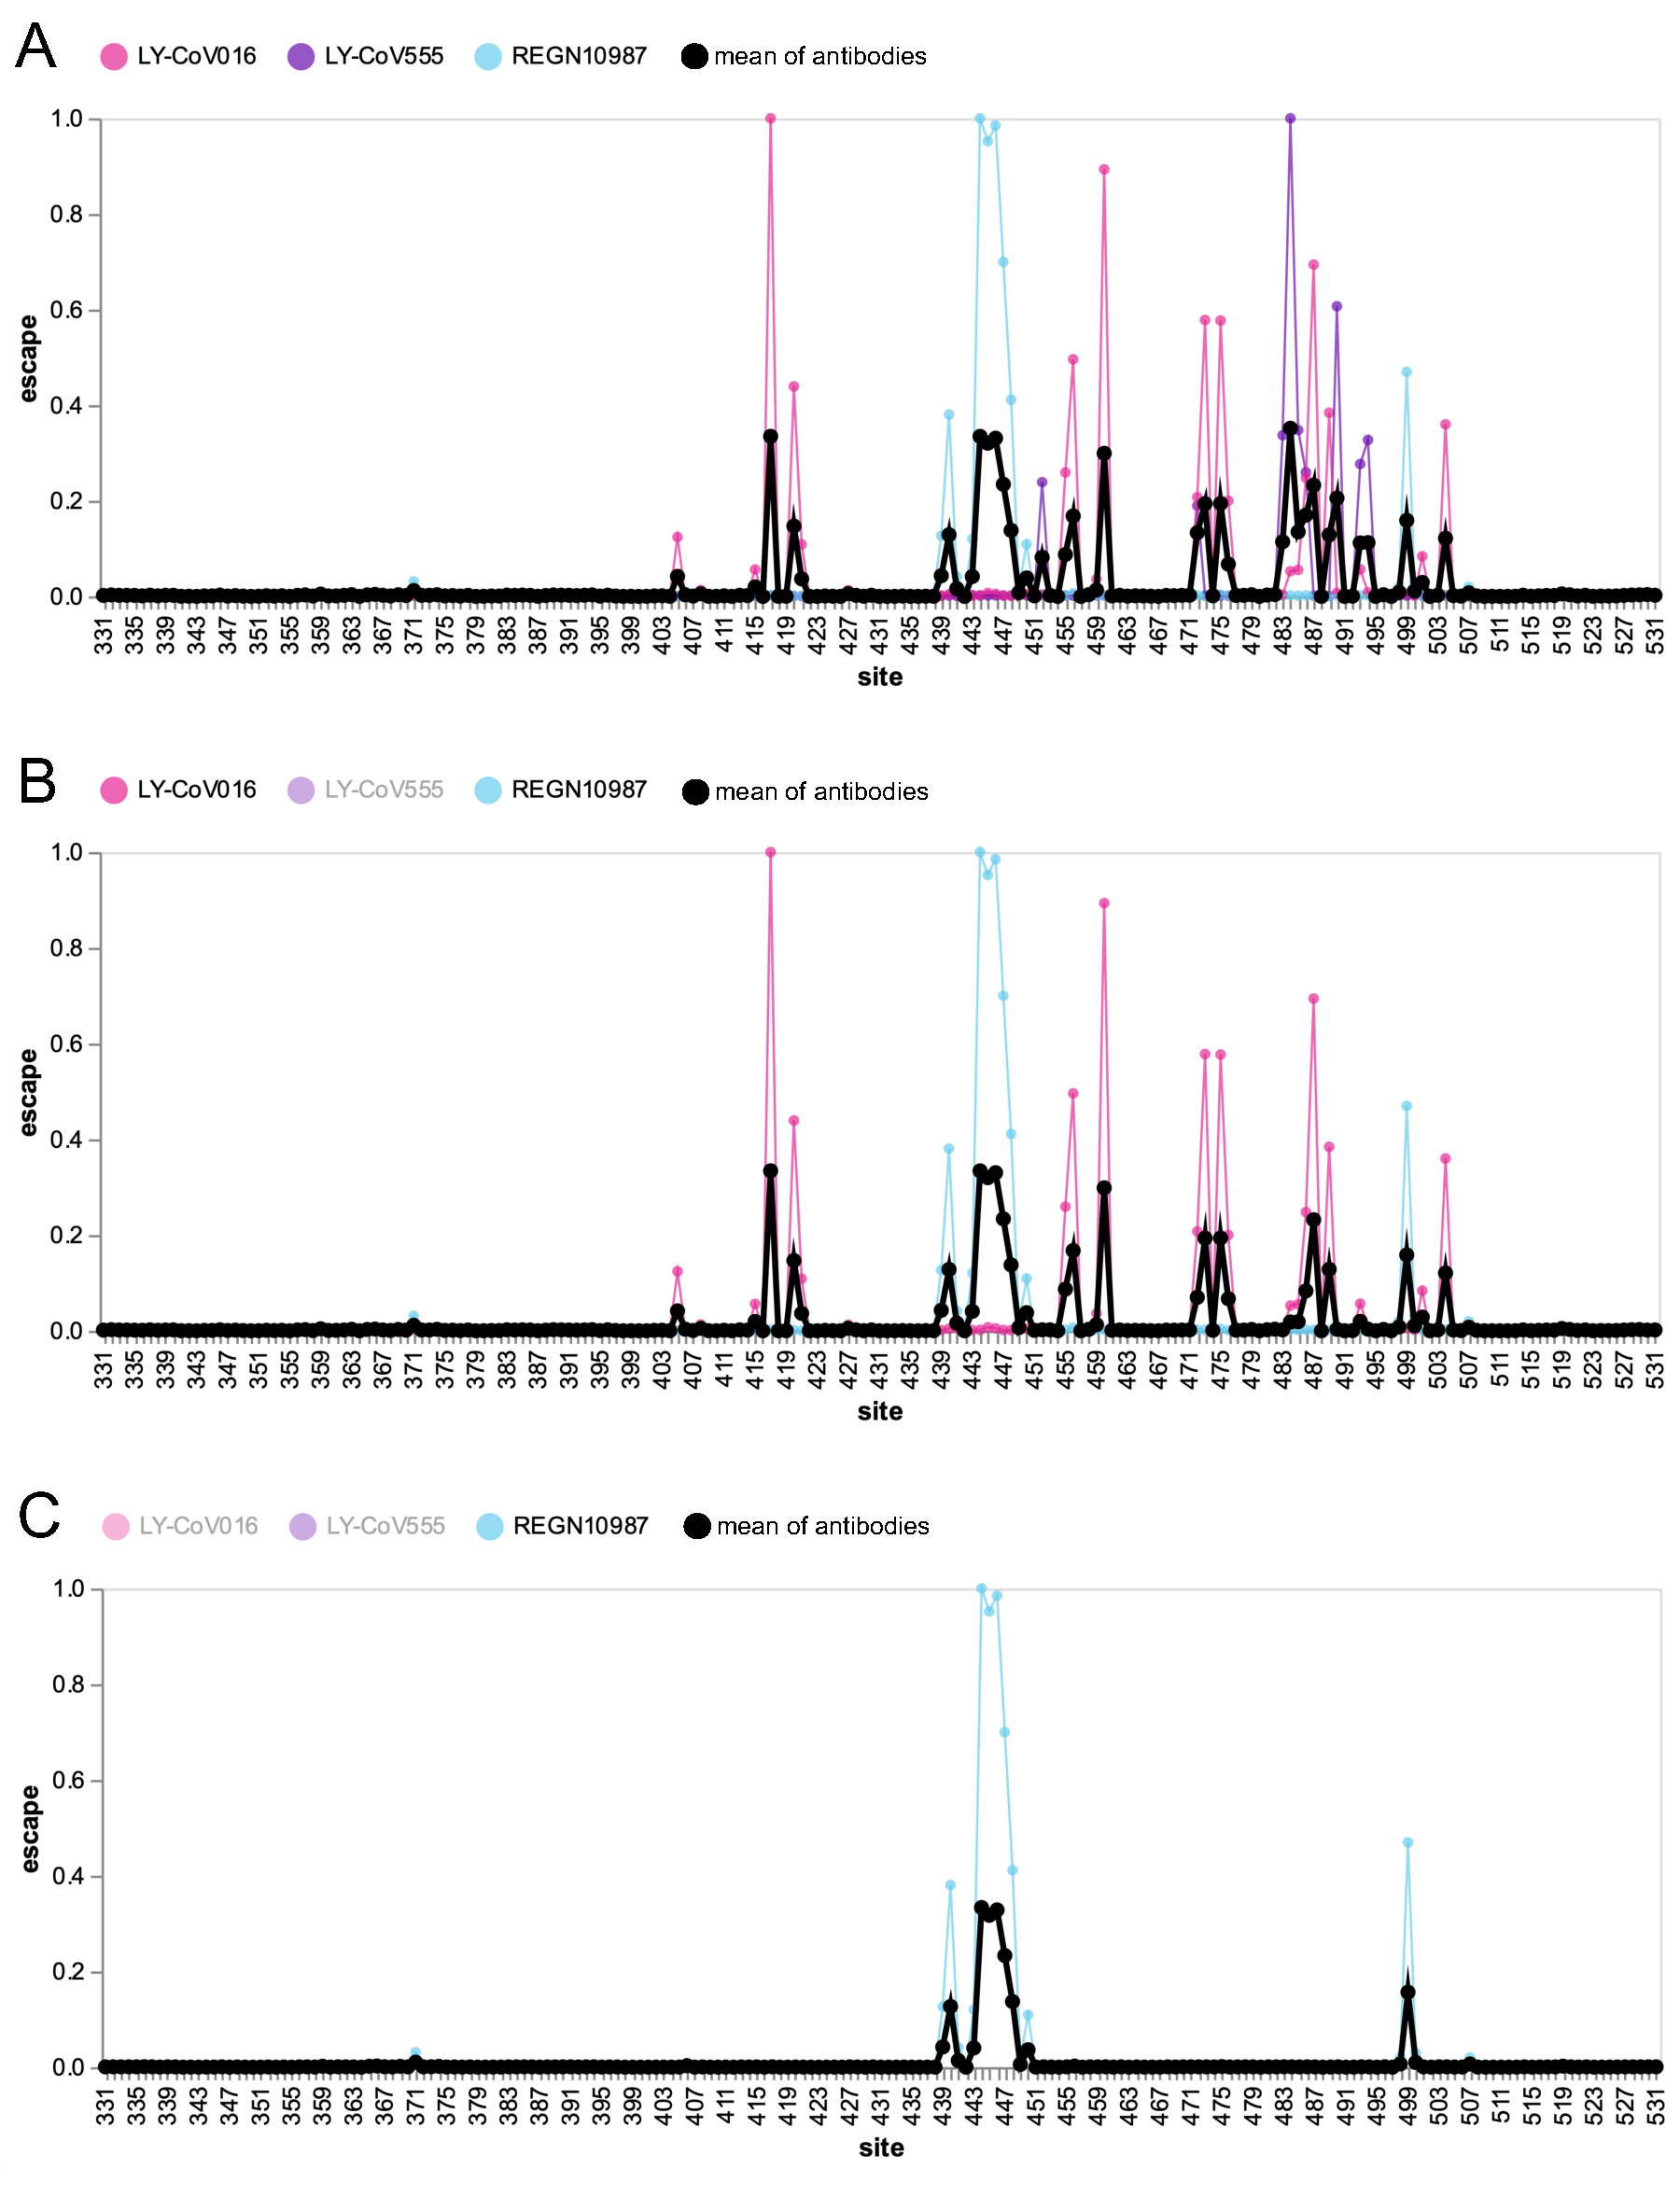
\includegraphics[width=0.71\textwidth]{figures/mini_example/mini_example.pdf} 

\caption{
Escape map for a hypothetical polyclonal mix consisting of an equipotent mixture of three monoclonal antibodies targeting distinct epitopes on the SARS-CoV-2 RBD.
{\bf (A)} Experimentally measured escape maps for three antibodies, and the mean of these maps (thick black line).
Each point on the x-axis represents a site in the RBD, and the y-axis represents the total measured escape by all mutations at that site scaled so the maximum for each antibody is one.
{\bf (B)} Escape map if the contribution of antibody LY-CoV555 is ablated.
{\bf (C)} Escape map if the contributions of antibodies LY-CoV555 and LY-CoV016 are ablated.
An interactive version of this figure is at \url{https://jbloomlab.github.io/SARS2_RBD_Ab_escape_maps/mini-example-escape-calc/}.}
\label{fig:mini_example}
\end{SCfigure*}

\subsection{Aggregating deep mutational scanning data for 33 human antibodies yields a realistic escape calculator}
%The toy example in the previous section illustrates how experimental data for individual antibodies can be combined to yield an escape map for a hypothetical polyclonal antibody mix.
To create an escape map for an antibody mix that more realistically represents actual human sera, we aggregated previously generated deep mutational scanning data for 33 neutralizing antibodies elicited by SARS-CoV-2.
These antibodies were isolated from a variety of patient cohorts within the first year of the pandemic (see Methods for details).
An assumption of the analysis that follows is that an equipotent mixture of these 33 antibodies represents the neutralizing activity of human sera; we emphasize that this assumption is imperfect since in reality the antibodies were chosen for prior study for a variety of ad hoc reasons.
The escape maps for all the individual antibodies can be interactively interrogated at \url{https://jbloomlab.github.io/SARS2_RBD_Ab_escape_maps/}.

\begin{SCfigure*}[][]
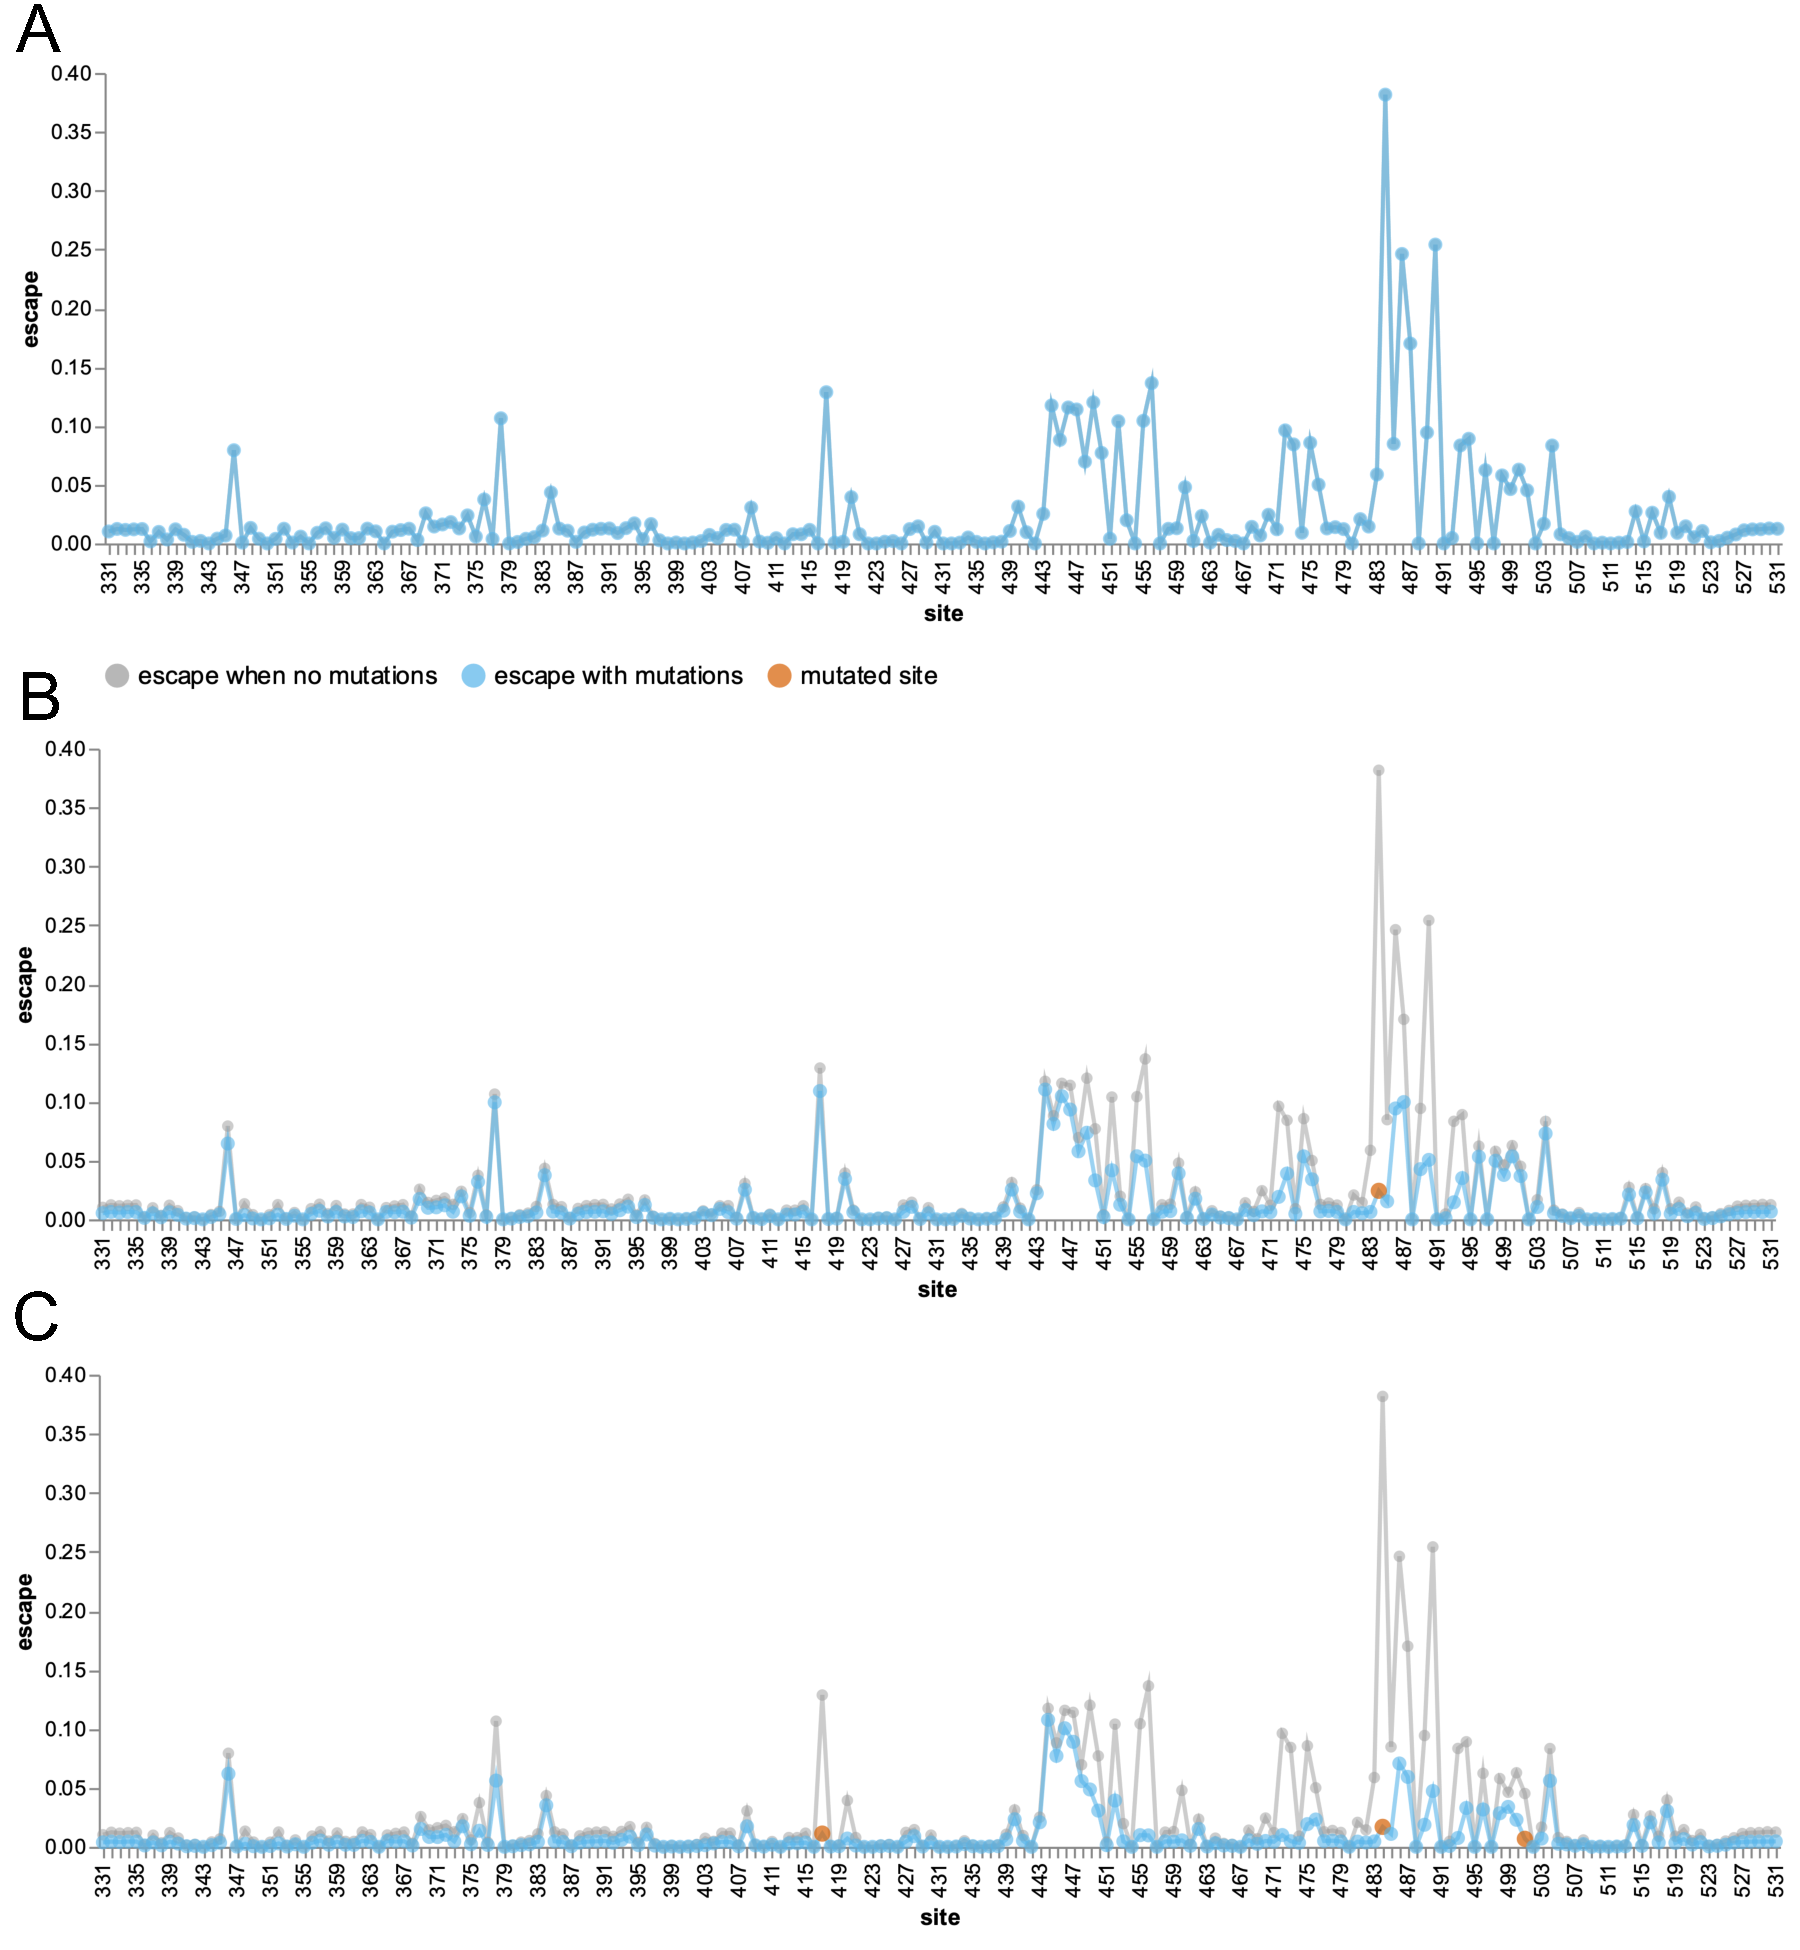
\includegraphics[width=0.8\textwidth]{figures/escape_calc/escape_calc.pdf}
\caption{
An escape calculator generated by aggregating deep mutational scanning for 33 neutralizing antibodies targeting the SARS-CoV-2 RBD.
{\bf (A)} The blue line shows the extent of escape mediated by mutations at each site, as estimated by simply averaging the data for all the individual antibodies.
{\bf (B)} The blue line shows escape map after a mutation to site 484 (red point) ablates recognition by antibodies strongly targeting that site, while the gray line shows the original escape map in the absence of any mutations.
{\bf (C)} The escape map after mutating sites 417, 484, and 501 (the three RBD sites mutated in the Beta variant).
An interactive version of this figure is at \url{https://jbloomlab.github.io/SARS2_RBD_Ab_escape_maps/escape-calc/}.}
\label{fig:escape_calc}
\end{SCfigure*}

The overall polyclonal escape map generated by averaging the data for all 33 antibodies is in Figure \ref{fig:escape_calc}A.
As in the toy three-antibody example in the previous subsection, there are peaks at  sites 417, 484, and 444--446.
However, the peak at 484 is now larger than any other peak, reflecting the fact that antibodies targeting the class 2 epitope containing E484 are immunodominant in the human antibody response to early SARS-CoV-2 strains~\citep{yuan2020structural,robbiani2020convergent,greaney2021comprehensive,greaney2021mapping}.
In addition, there are smaller peaks at a variety of other sites, reflecting the fact that each antibody has a somewhat idiosyncratic epitope (Figure \ref{fig:escape_calc}A).

We can follow the principle outlined in the toy example in the previous subsection to calculate the expected polyclonal escape map \emph{after} mutating sites in the RBD.
Specifically, we reduce the contribution of each antibody by an amount that scales with how strongly that antibody targets each mutated site (see Methods for mathematical details).
For instance, the blue lines in Figure~\ref{fig:escape_calc}B show the polyclonal escape map after mutating site 484.
Mutating site 484 obviously drops the contribution of that site, but it also decreases the contribution of other sites such as 490 that are commonly targeted by antibodies with epitopes that include site 484.
In contrast, mutating site 484 has minimal effect on the polyclonal escape map at sites like 417 or 444--446, since those sites are generally targeted by antibodies that are unaffected by mutations at site 484.

We can also calculate the expected effects of compound mutations.
Figure~\ref{fig:escape_calc}C shows the polyclonal escape map after mutating all three RBD sites that are changed in the Beta variant (sites 417, 484, and 501).
This polyclonal escape map has lost contributions not only from the mutated sites, but also sites that form common epitopes with 417 or 484 (e.g., sites 455, 456, 486, and 490).
However, the escape map still has major contributions from antibodies targeting sites like 444--446, since such antibodies are generally unaffected by mutations at sites 417, 484, or 501.

We recommend the reader explores the interactive escape calculator at \url{https://jbloomlab.github.io/SARS2_RBD_Ab_escape_maps/escape-calc/}, to perform calculations like those in Figure~\ref{fig:escape_calc} for arbitrary combinations of mutated RBD sites.
Such visual exploration of different combinations of mutations provides an intuitive sense of the antigenic structure of the RBD.

\subsection{The escape calculations correlate well with neutralization assays on SARS-CoV-2 variants}
We can also define a quantitative score that summarizes the polyclonal antibody binding that remains after an arbitrary combination of RBD mutations.
This score is defined using the same principle as the site-wise escape calculator in the previous subsection: we reduce the contribution of each antibody by an amount that scales with how strongly it is escaped by each mutated site, and define the overall score as the fraction of all antibody contributions that remain after the mutations (see Methods for details).
This calculation is implemented in the interactive calculator at \url{https://jbloomlab.github.io/SARS2_RBD_Ab_escape_maps/escape-calc/}, and returns a score that ranges from one (no mutations affect binding of any antibodies) to zero (all antibodies fully escaped).

\begin{SCfigure*}[][]
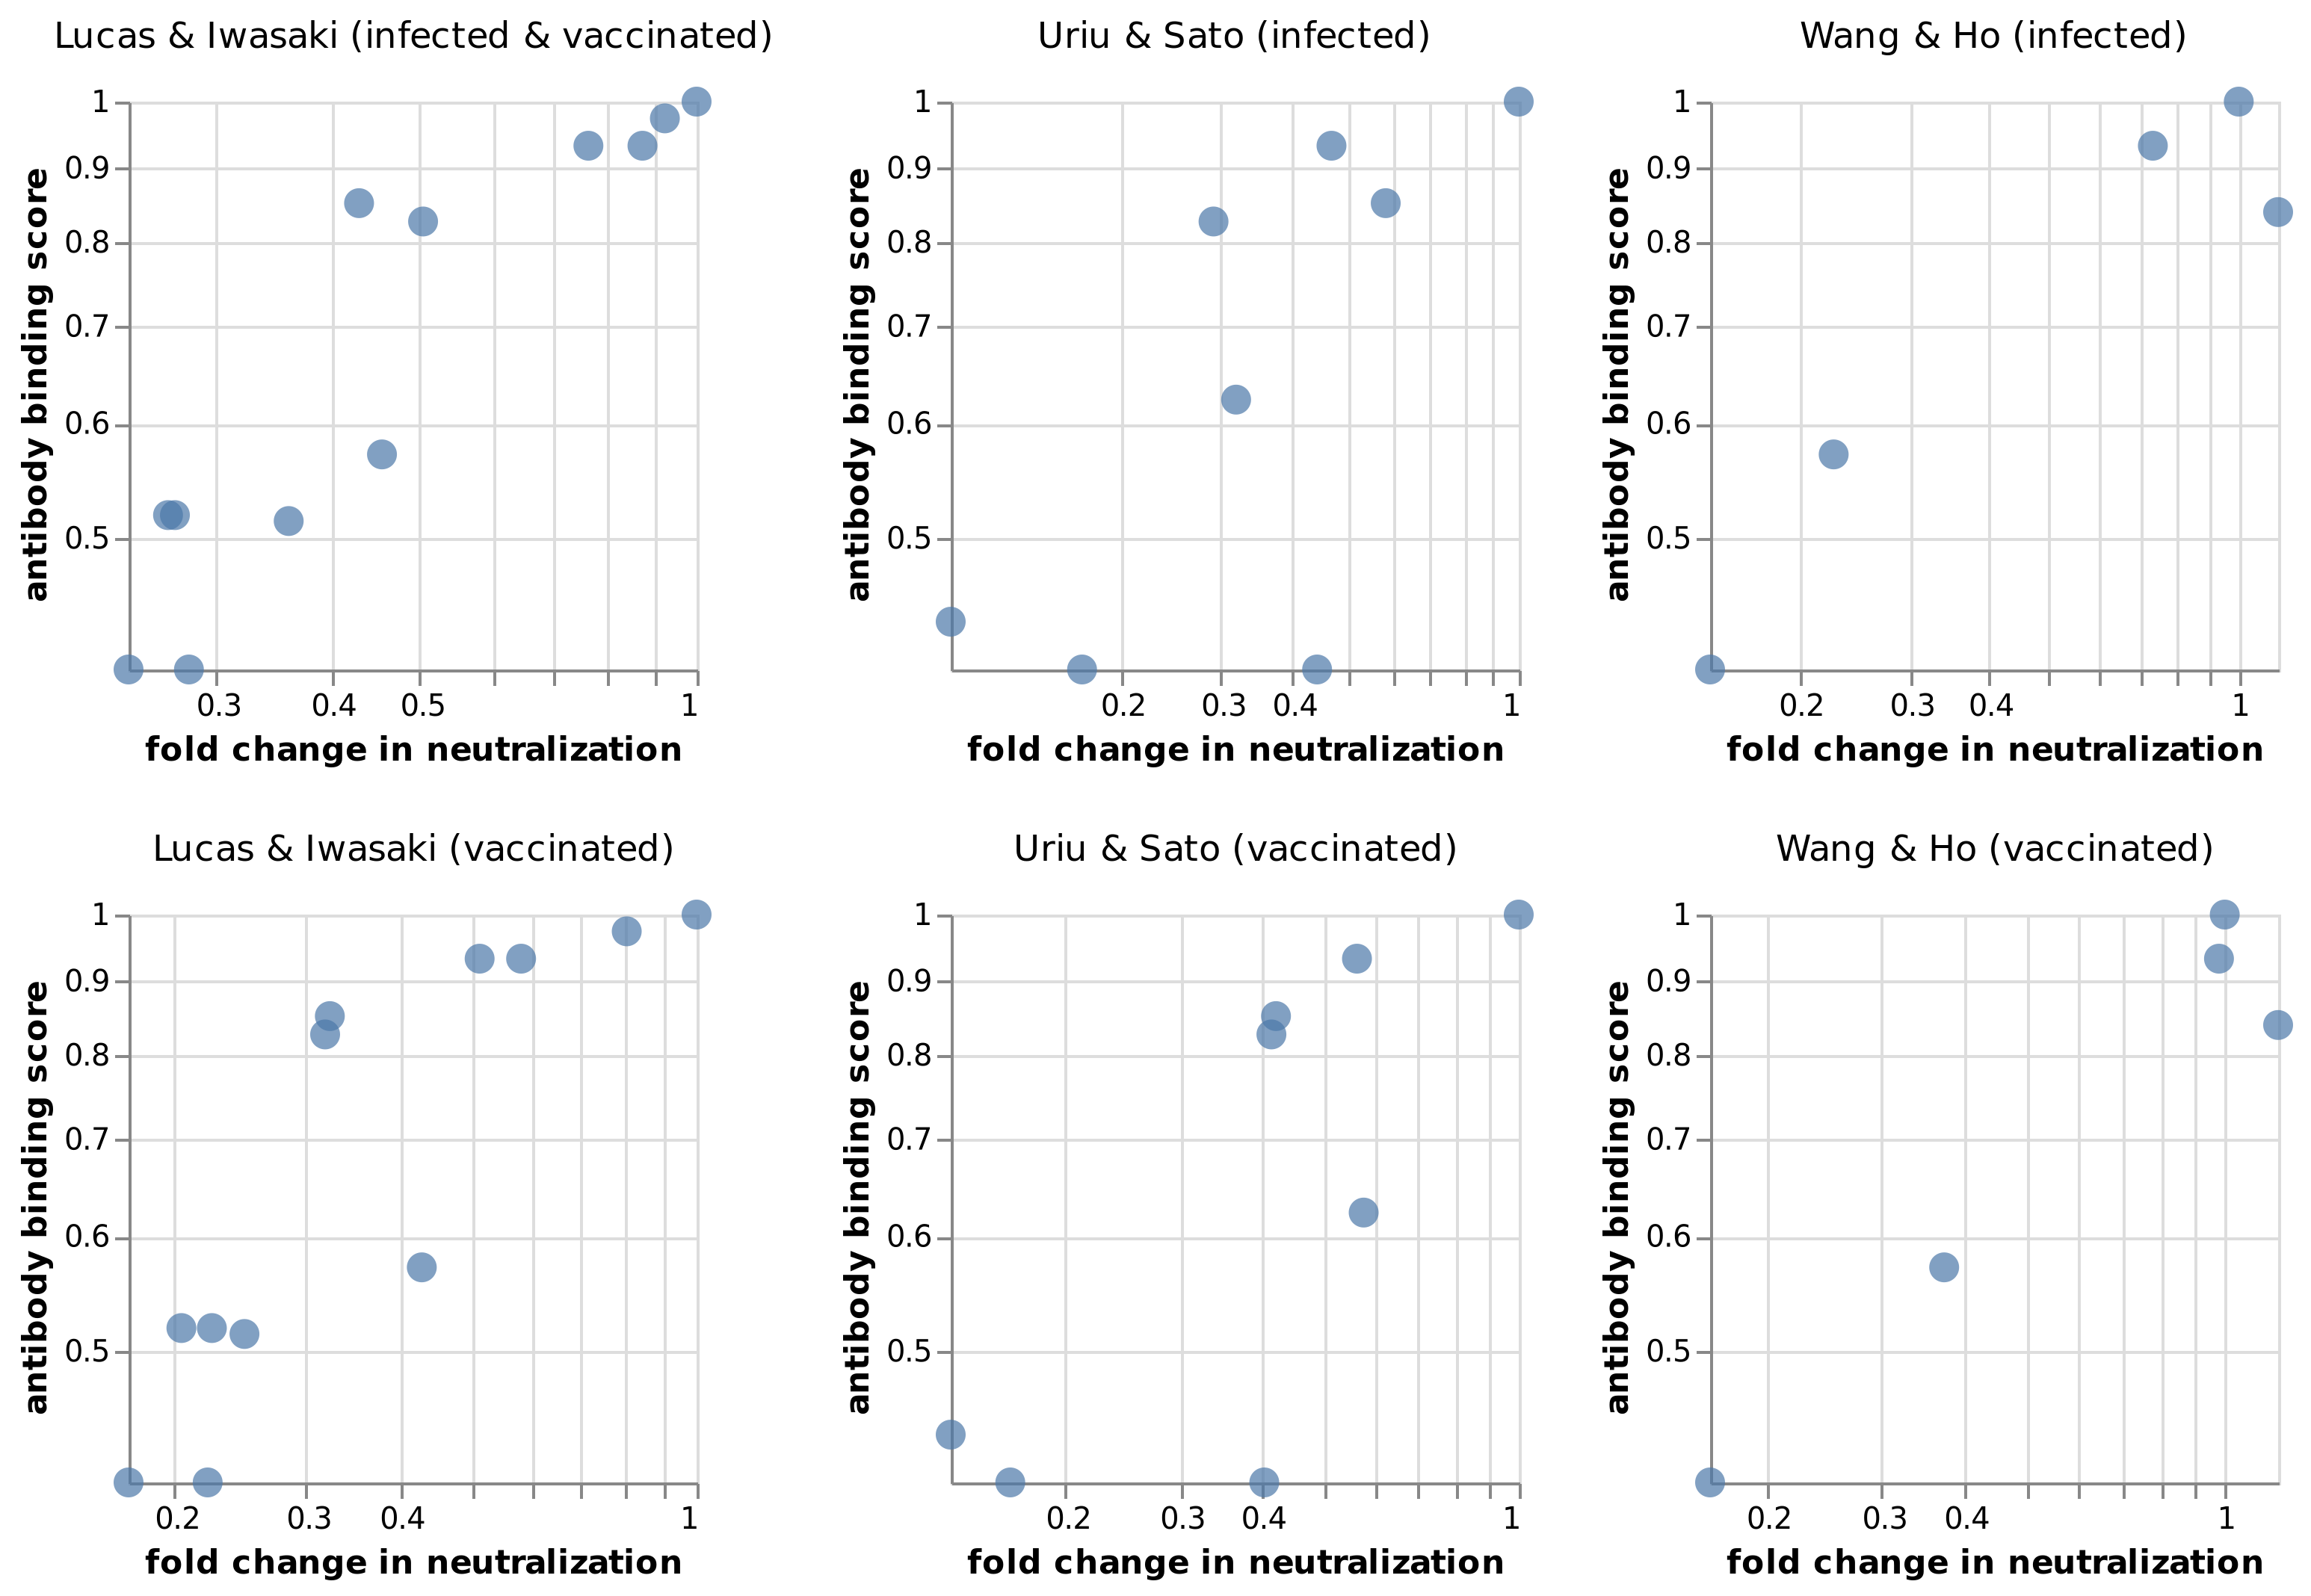
\includegraphics[width=0.7\textwidth]{../results/neut_studies/neut_studies.png}
\caption{Correlation of escape scores from the calculator with experimentally measured fold changes in neutralization IC50 values for SARS-CoV-2 variants and mutants.
The experimental data of \citet{lucas2021impact} was generated using live virus and sera from vaccinated individuals who were (top) or were not (bottom) previously infected with SARS-CoV-2.
The experimental data of \citet{uriu2021neutralization} and \citet{wang2021antibody} was generated using pseudovirus against convalescent (top) or vaccine (bottom) sera, with the vaccine sera from the Pfizer BNT162b2 or Moderna mRNA-1273 vaccines, respectively. 
The plotted fold changes in neutralization represent the geometric means over all subjects in each cohort.
}
\label{fig:neut_studies}
\end{SCfigure*}

To test how these escape-calculator scores compare to actual experimentally measured neutralization titers, we collated neutralization data from three previously published studies~\citep{lucas2021impact,uriu2021neutralization,wang2021antibody}, each of which characterized sera from two patient cohorts against a variety of SARS-CoV-2 variants and mutants.
One can imagine many reasons why the escape-calculator scores might differ from the real neutralization titers: the calculator only considers RBD mutations and neglects those in other domains such as the NTD, the antibodies used by the calculator might not accurately reflect the real mix in polyclonal sera, etc.
But despite all these potential caveats, the escape-calculator scores correlate quite well with the measured neutralization titers across all studies and cohorts (Figure~\ref{fig:neut_studies}).
Therefore, the simple and intuitive approach used by the calculator seems to accurately reflect the dominant features of polyclonal antibody escape in the RBD.

\subsection{The escape calculator suggests extensive antigenic change in the new Omicron variant}
We applied the escape calculator to the recently reported Omicron variant, which has 15 mutated sites in its RBD~\citep{?}.
The overall escape-calculator binding score for the polyclonal antibody mix is much lower for the Omicron variant than any other SARS-CoV-2 variants of concern (Figure~\ref{fig:Omicron}A).
The Omicron variant's calculated score is roughly equivalent to that of a polymutant spike (PMS20) that was artificially engineered in a pseudovirus by \citet{schmidt2021high} to maximize escape from polyclonal serum antibodies.
For comparison, \citet{schmidt2021high} measured that neutralization titers against this artificial PMS20 spike were reduced by $\sim$20- to $\sim$80-fold for sera from various cohorts of vaccinated and infected individuals.

\begin{figure*}
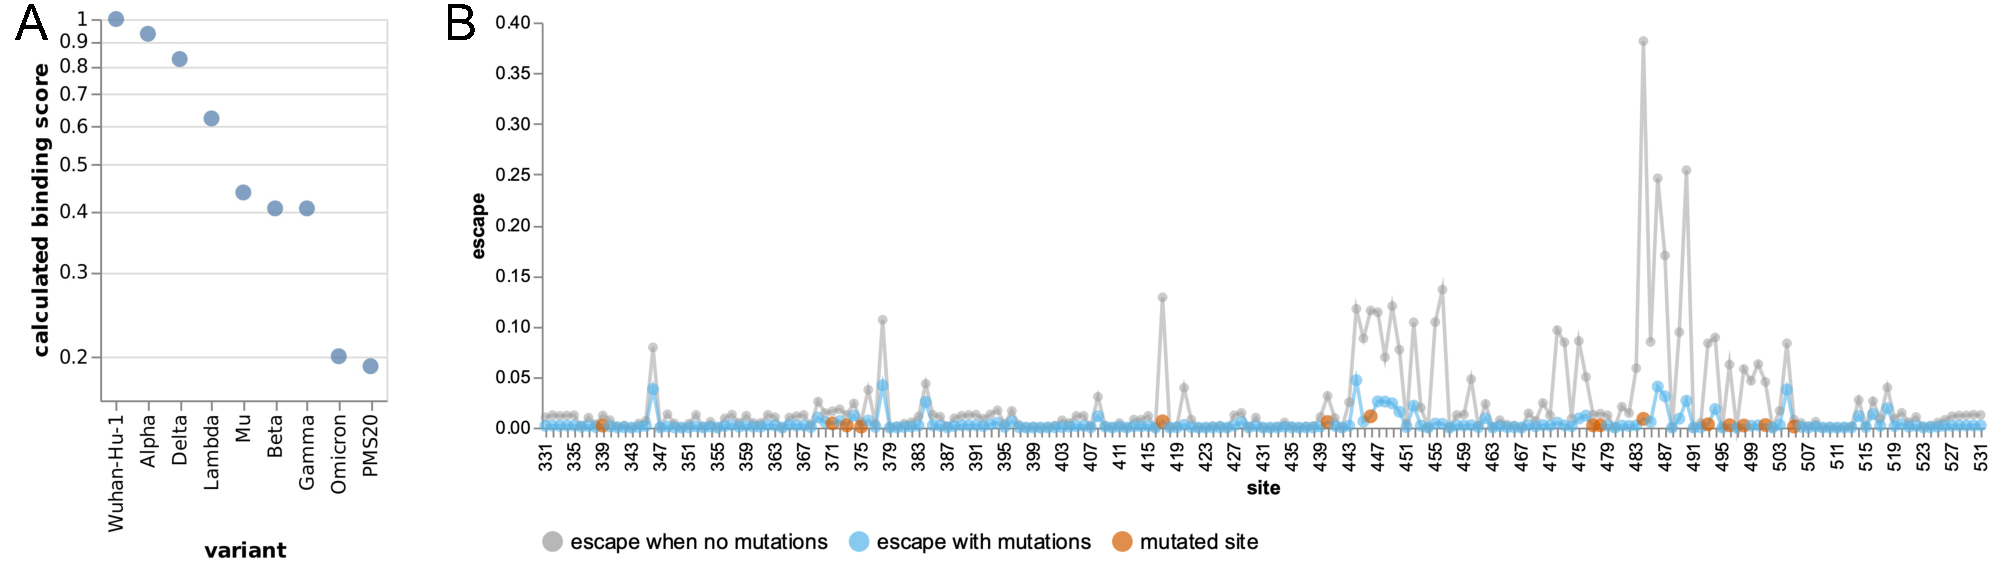
\includegraphics[width=\linewidth]{figures/Omicron/Omicron.pdf}
\caption{Escape calculations for the Omicron variant.
{\bf (A)} The calculated binding scores for SARS-CoV-2 variants and the artificial polymutant spike (PMS20) generated by \citet{schmidt2021high}.
Scores of one indicate no mutations affect binding, and scores of zero indicate no antibody binding remains.
{\bf (B)} The calculated escape map for the Omicron variant's RBD (blue) compared to an unmutated RBD (gray), with sites of mutations in the Omicron variant in red.
}
\label{fig:Omicron}
\end{figure*}

The site-level escape map for the Omicron variant's RBD is shown in Figure~\ref{fig:Omicron}B.
That map shows that the Omicron RBD has lost most peaks of antibody binding relative to the original RBD.
Exploration of the mutations using the interactive calculator at \url{https://jbloomlab.github.io/SARS2_RBD_Ab_escape_maps/escape-calc/} indicates that the mutations at sites 417, 446, and 484 are the biggest drivers of this antigenic change, although other mutations also contribute.
The residual peaks in the map suggests that the remaining antibody activity against the Omicron variant RBD could be further eroded by mutations at sites like 346, 378, 444, and 504.

\section{Discussion}


{\small

\section{Methods}
\subsection{Code and data availability}

\subsection{Mutations in Omicron variant and spike polymutant PMS20}
Omicron has mutations at the following 15 RBD sites: 339, 371, 373, 375, 417, 440, 446, 477, 478, 484, 493, 496, 498, 501, and 505.
PMS20 has mutations at the following 8 RBD sites: 346, 417, 440, 445, 455, 475, 484, and 501.


\section{Acknowledgments}
{\color{red} GISAID}
JDB is an Investigator of the Howard Hughes Medical Institute.

\section{Competing interests}
JDB consults for Moderna and Flagship Labs 77, and is an inventor on a Fred Hutch licensed patents related to deep mutational scanning of viral proteins.

}

\bibliography{references}

\end{document}
